\documentclass[titlepage,12pt,a4paper,times]{book}

\usepackage[utf8]{inputenc}
\usepackage[portuguese]{babel}
% substituir linha anterior por 
% \usepackage[english]{babel} 
% se o relatório for escrito na língua inglesa.
\usepackage[T1]{fontenc}
\usepackage{makeidx}
\usepackage{xspace}
\usepackage[labelfont=bf]{caption}
\usepackage{graphicx,color,times}
\usepackage{subcaption}
\usepackage{fancyhdr}
\usepackage[hyphens]{url}
% \usepackage{pxfonts}
% \usepackage{times}
% \usepackage{mathptm}
% \usepackage{amssymb}
% \usepackage{amsfonts}
\usepackage{amsmath}
\usepackage{latexsym}
\usepackage[printonlyused]{acronym}
\usepackage{float}
\usepackage{listings}
\usepackage{tocbibind}
\usepackage{wrapfig}
\usepackage{natbib}
\usepackage{hyperref}
\usepackage[shortlabels]{enumitem}
% \usepackage{glossaries}
% \makeglossaries

\renewcommand{\ttdefault}{phv}

\pagestyle{fancy}
\renewcommand{\chaptermark}[1]{\markboth{#1}{}}
\renewcommand{\sectionmark}[1]{\markright{\thesection\ #1}}
\fancyhf{} \fancyhead[LE,RO]{\bfseries\thepage}
\fancyhead[LO]{\bfseries\rightmark}
\fancyhead[RE]{\bfseries\leftmark}
\renewcommand{\headrulewidth}{0.5pt}
\renewcommand{\footrulewidth}{0pt}
\addtolength{\headheight}{0.5pt}
\setlength{\marginparsep}{0cm}
\setlength{\marginparwidth}{0cm}
\setlength{\marginparpush}{0cm}
\addtolength{\hoffset}{-1.0cm}
\addtolength{\oddsidemargin}{\evensidemargin}
\addtolength{\oddsidemargin}{0.5cm}
\addtolength{\evensidemargin}{-0.5cm}


% NEW COLORS
\definecolor{dark}{gray}{0.25}
\definecolor{lgray}{gray}{0.9}
\definecolor{dkblue}{rgb}{0,0.13,0.4}
\definecolor{dkgreen}{rgb}{0,0.6,0}
\definecolor{gray}{rgb}{0.5,0.5,0.5}
\definecolor{mauve}{rgb}{0.58,0,0.82}

\lstset{ %
  language=C,                    basicstyle=\footnotesize,
  numbers=none,                  numberstyle=\tiny\color{gray}, 
  stepnumber=1,                  numbersep=5pt,
  backgroundcolor=\color{white}, showspaces=false,
  showstringspaces=false,        showtabs=false,
  frame=single,                  rulecolor=\color{black},
  tabsize=2,                     captionpos=b,
  breaklines=true,               breakatwhitespace=false,
  title=\lstname,                keywordstyle=\color{blue},
  commentstyle=\color{dkgreen},  stringstyle=\color{mauve},
  escapeinside={\%*}{*)},        morekeywords={*},
  belowskip=0cm
}

\renewcommand{\lstlistingname}{Excerto de Código}
\renewcommand{\lstlistlistingname}{Lista de Excertos de Código}% 

\begin{document}


\thispagestyle{empty}
\setcounter{page}{-1}

\begin{center}
\begin{Huge}
\textbf{Universidade da Beira Interior}
\end{Huge}
\end{center}

\begin{center}
\begin{Huge}
Departamento de Informática
\end{Huge}
\end{center}

\vspace{0,07cm}
\begin{figure}[!htb]
\centering

\includegraphics[width=191pt]{ubi-fe-di.png}
\end{figure}

\vspace{0.5cm}
\begin{center}
\begin{Large}
\textbf{Aspetos profissionais, legais e éticos na Gestão de Dados em SGBD}
\end{Large}
\end{center}


\vspace{0.5cm}
\begin{center}
\begin{normalsize}
\begin{large}
Elaborado por:
\end{large}
\end{normalsize}
\end{center}

\vspace{0.2cm}
\begin{center}
\begin{large}
\textbf{João Brito, M9984 \\ Luís Pereira, M10156 \\ Carlos Esteves, E10304}
\end{large}
\end{center}

\vspace{0,5cm}
\begin{center}
\begin{normalsize}
\begin{large}
Orientador:
\end{large}
\end{normalsize}
\end{center}

\vspace{0.2cm}
\begin{center}
\begin{large}
\textbf{Professor Doutor Rui Cardoso}
\end{large}
\end{center}



\vspace{0.5cm}
\begin{center}
\begin{normalsize}
9 de janeiro de 2020
\end{normalsize}
\end{center}


\clearpage{\thispagestyle{empty}\cleardoublepage}

\frontmatter

\chapter*{Agradecimentos}
\label{chap:ack}

A conclusão deste trabalho não teria sido possível sem a imprescindível ajuda do meu orientador de projeto, o Professor Doutor Hugo Proença. Os seus conselhos e ensinamentos nortearam este projeto.\newline

\noindent De seguida, quero manifestar o meu apreço pelo apoio e companheirismo demonstrados pelos meus colegas de curso e amigos próximos.\newline

\noindent Por último, mas não menos importante, gostaria de agradecer o suporte incondicional prestado pela minha família durante o meu percurso académico.

\clearpage{\thispagestyle{empty}\cleardoublepage}


\tableofcontents

\clearpage{\thispagestyle{empty}\cleardoublepage}

\listoffigures

% Se não existirem tabelas, comentar as seguintes linhas
\clearpage{\thispagestyle{empty}\cleardoublepage}
\listoftables

% Se existirem trechos de código, descomentar as seguintes linhas
% \clearpage{\thispagestyle{empty}\cleardoublepage}
% \lstlistoflistings

\clearpage{\thispagestyle{empty}\cleardoublepage}
\chapter*{Acrónimos}
\label{chap:acro}

\begin{acronym}[SGBD]
  \acro{BD}{\emph{Base de Dados}}
  \acro{CNPD}{\emph{Comissão Nacional de Protecção de Dados}}
  \acro{RGPD}{\emph{Regulamento Geral sobre a Proteção de Dados}}
  \acro{SGBD}{\emph{Sistema de Gestão de Bases de Dados}}
\end{acronym}

% \clearpage{\pagestyle{empty}\cleardoublepage}
% \chapter*{Glossário}
\makeglossaries

\newglossaryentry{.NET Framework}
{
  name={.NET Framework},
  description={É uma plataforma para desenvolvimento e funcionamento de aplicações desenvolvida pela Microsoft.}
}

\newglossaryentry{ASP.NET}
{
  name={ASP .Net},
  description={É uma plataforma da Microsoft para o desenvolvimento de aplicações Web e é o sucessor da tecnologia ASP.}
}

\newglossaryentry{CS}
{
  name={C\#},
  description={Lê-se \textit{C Sharp} e é uma linguagem de programação orientada a objectos, desenvolvida pela Microsoft, inicialmente para a plataforma .NET. O C\# é inspirado na junção entre as linguagens C++ e Java.}
}


\newglossaryentry{Java}
{
  name={JAVA},
  description={É uma linguagem de programação orientada a objectos, desenvolvida pela Sun Microsystems na década de 90. Hoje pertence à empresa Oracle.}
}


\newglossaryentry{OpenDMTP}
{
  name={OpenDMTP},
  description={\textit{Open Device Monitoring and Tracking Protocol} é um protocolo e uma \textit{framework} abertos que permite a comunicação bidireccional entre servidores e clientes através da internet.}
}


\newglossaryentry{OpenGTS}
{
  name={Open GTS},
  description={É o primeiro projecto \textit{Open Source} \textit{Web-Based} para controlo de frotas por GPS.}
}


\newglossaryentry{VS2010}
{
  name={Visual Studio 2010},
  description={\textit{Microsoft Visual Studio 2010} é um sistema de desenvolvimento desenvolvido pela Microsoft e é dedicado ao Framework .NET, que contem um conjunto de ferramentas de desenvolvimento projectadas para auxiliar os programadores a enfrentarem desafios complexos.}
}


\newglossaryentry{WebS}
{
	name={Web Service},
	description={Web services são aplicações modulares auto-descritas e auto-contidas, que permitem a integração de sistemas e a comunicação entre aplicações de diferentes tipos.}
}


\newglossaryentry{WebBased}
{
	name={Web Based},
	description={Aplicação desenvolvida para a Web.}
}

\newglossaryentry{Roaming}
{
	name={Roaming},
	description={Define a possibilidade de um utilizador de uma determinada rede obter rede/conecção fora da área geográfica onde foi registado.}
}


\newglossaryentry{Smartphone}
{
	name={Smartphone},
	description={Smartphone é um telefone móvel que contem muitas das principais tecnologias de comunicação e serviços que existem nos computadores pessoais, como acesso a e-mails, serviços de mensagens instantâneas, internet, GPS, entre outros.}
}

\newglossaryentry{TCPIP}
{
	name={TCP/IP},
	description={É um conjunto de protocolos de comunicação entre computadores ligados rede. O nome TCP/IP surge da união entre dois protocolos: o TCP (Transmission Control Protocol) e o protocolo IP (Internet Protocol).}
}

\newglossaryentry{Firewall}
{
	name={Firewall},
	description={É o nome criado para definir um dispositivo para uma rede de computadores que tem como objectivo criar uma política de segurança num determinado ponto de controlo da rede.}
}

\newglossaryentry{JavaScript}
{
	name={JavaScript},
	description={É uma linguagem de programação baseada na linguagem de programação ECMAScript. Actualmente é a linguagem de programação mais utilizada em \textit{``Client-Side''} nos \textit{browsers}.}
}

\newglossaryentry{Flash}
{
	name={Flash},
	description={Desenvolvido pela Macromedia, o Flash é um software utilizado para criação de animações interactivas que funcionam incorporadas em \textit{Browsers}, \textit{Desktop}, \textit{Smartphones}, \textit{Tablets}, e Televisores.}
}


\newglossaryentry{StoredProcedure}
{
	name={Stored Procedure },
	description={É o nome dado a um conjunto de comandos numa base de dados de forma a simplificar a sua utilização.}
}

\newglossaryentry{SQLS}
{
	name={SQL Server 2008},
	description={É um sistema de gestão de base de dados relacional criado pela Microsoft.}
}

\newglossaryentry{Firm}
{
	name={Firmware},
	description={É o conjunto de instruções operacionais programadas directamente no \textit{hardware} de um equipamento electrónico.}
}

\newglossaryentry{browser}
{
	name={Browser},
	description={É um programa de computador que possibilita aos utilizadores uma interacção com documentos virtuais da Internet, também conhecidos como páginas Web.}
}



\clearpage{\thispagestyle{empty}\cleardoublepage}
    
\mainmatter
\acresetall
%Indentação
\setlength{\parskip}{1em}
\setlength{\parindent}{0pt}

\chapter{Introdução}
\label{chap:intro}

\section{Enquadramento}
\label{sec:amb}

Este projeto foi realizado no contexto da unidade curricular de Tecnologias de Base de Dados, enquadrada no primeiro ano de Mestrado em Engenharia Informática da Universidade da Beira Interior, no ano letivo 2019/2020.

\section{Motivação}
\label{sec:mot}

O projeto foi proposto e será avaliado pelo professor docente Rui Cardoso. Visa a exploração de aspetos legais, éticos e profissionais na gestão de dados. Estes princípios serão, ainda, discutidos no âmbito de um \ac{SGBD}.

\section{Objetivos}
\label{sec:obj}
O presente projeto procurará expor a temática da gestão de dados em várias vertentes. Do ponto de vista profissional, podem ser considerados aspetos puramente técnicos (i.e. como são, efetivamente, guardados os dados). A título legal, será procurado o auxílio da legislação em vigor. Por fim, o caráter ético na gestão de informação terá destaque neste documento teórico, nunca esquecendo a importância que tem (ou deve ter) na prática.


\section{Constituição do grupo}
\label{sec:const_grupo}
A constituição do grupo de trabalho a que se deve a realização deste documento, e respetivo projeto, foi da responsabilidade dos próprios elementos, que se encontram aqui descritos:
\begin{itemize}
    \item João Brito, M9984;
    \item Luís Pereira, M10156;
    \item Carlos Esteves, E10304.
\end{itemize}

\section{Organização do Documento}
\label{sec:organ}
O presente documento encontra-se dividido em sete secções principais, nomeadamente:
\begin{enumerate}
    \item Introdução - é feita uma apresentação do projeto, identificando os objetivos e o seu âmbito;
    \item Gestão de dados: onde começam e acabam os limites? - são introduzidas questões e problemáticas associadas à gestão indevida de dados;
    \item Como dar garantias ao utilizador de que a gestão de dados é bem feita? - é abordada a necessidade de transparência de uma empresa ou entidade para com os seus utilizadores;
    \item Legislação existente - é feita uma revisão de algumas leis e entidades relevantes;
    \item Mecanismos de proteção de dados - são explorados aspetos mais técnicos no âmbito da gestão de dados num \ac{SGBD};
    \item Falhas e abusos na gestão de dados - são referidos alguns exemplos de uma gestão de dados incorreta;
    \item Conclusão e Trabalho Futuro - apresentam-se conclusões derivadas do trabalho desenvolvido, bem como algumas notas sobre possíveis melhorias ou tópicos passíveis de serem explorados.
\end{enumerate}
\clearpage{\thispagestyle{empty}\cleardoublepage}
\chapter{Modelos de Aprendizagem Profunda}
\label{chap:redes-neuronais-convolucionais}

\section{Introdução}
\label{chap2:sec:intro}
O nosso cérebro processa constantemente o ambiente que nos rodeia. Durante todo o processo de aprendizagem e crescimento por que o ser humano passa, o cérebro cria regras que lhe permitem, entre muitas outras coisas, classificar objetos de forma quase instantânea. Este processo começa de forma supervisionada (os nossos pais classificam objetos, inicialmente desconhecido, por nós) levando a que criemos parâmetros que permitirão a identificação autónoma de futuras instâncias de qualquer objeto.\newline
\noindent 
\newline
\noindent Sabe-se que um neurónio recebe informação através das dendrites, processa o que recebeu e dispara um \textit{output} adequado. Trata-se, claramente, de uma simplificação daquele que é talvez um dos mecanismos mais fascinantes que a Ciência estuda. Contudo, serviu de base para que em 1943 o neurocientista  Warren McCulloch e o matemático Walter Pitts propusessem um neurónio artificial. A ideia base seria a mesma de um neurónio biológico, aliada à esperança de que muitas células simples seriam capazes de dar respostas complexas. 

\begin{figure}[h]
\centering
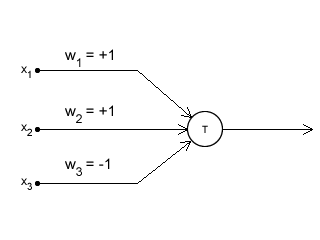
\includegraphics[width=155pt]{mp_neuron.png}
\caption{Modelo do neurónio artificial proposto por McCulloch e Pitts \cite{neuron_site}.}
\label{fig:mp_neuron}
\end{figure}

\section{Córtex Visual Primário}
\label{chap2:sec:cortex_visual}
Situado no Lobo Occipital, o Córtex Visual Primário (V1) é, a nível da visão, uma das regiões mais estudadas do cérebro. Sendo extremamente especializado na análise de objetos tanto em movimento como estáticos, possui um alto grau de reconhecimento de padrões.

\begin{figure}[h]
\centering
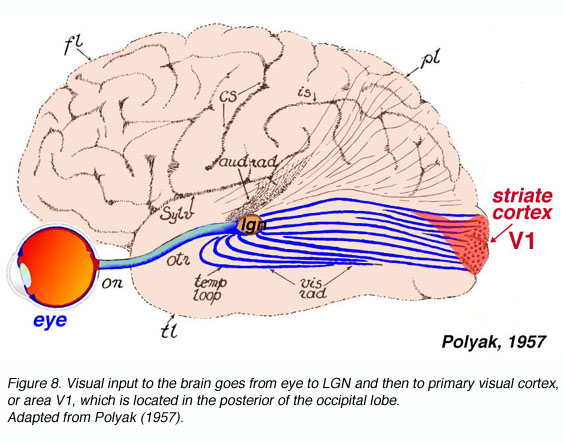
\includegraphics[width=150pt]{cortex.jpg}
\caption{Fluxo de informação desde o olho até ao Córtex Visual Primário \cite{cortex_site}.}
\label{fig:cortex}
\end{figure}

\noindent No decorrer do processamento de informação (figura \ref{fig:cortex}), o \textit{input} visual é obtido pela retina, com intervenção das suas células ganglionares, cones, bastonetes, células horizontais, células bipolares e células amácrinas. As terminações das células ganglionares agregam-se e surgem na parte posterior do olho já sob a forma do nervo ótico. A continuação deste nervo crucial para a Via Visual Primária, denominada de trato ótico, transporta a informação sensorial até ao \ac{NGL} - localizado no Tálamo, um importante centro nervoso.

\noindent Algum processamento é realizado nesta secção, destacando-se as células M (\textit{Magnocellular}), P (\textit{Parvocellular}) e K (\textit{Koniocellular}). Existem funções bem definidas e um grau de especialização diferenciador: os neurónios M são particularmente afetos à deteção de movimento; os neurónios P às caraterísticas espaciais (tamanho e forma) e os neurónios K a alguns aspetos da visão cromática.

\begin{figure}[h]
\centering
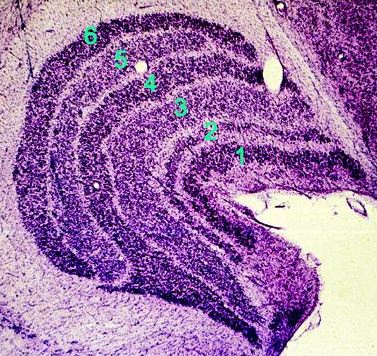
\includegraphics[width=115pt]{m_p_k_cells.jpg}
\caption{As seis camadas que compõe o \ac{NGL}: 1-2 (células M); 3-6 (células P) e as células K situam-se em zonas intermédias \cite{cells}.}
\label{fig:via_visual}
\end{figure}

\noindent Finalmente, esta informação filtrada e levemente tratada chega ao seu destino, o Córtex Visual Primário.

\noindent A partir dos estudos de Hubel e Weisel na década de 1960, foi possível perceber que os neurónios em V1 são excitados por caraterísticas tanto simples como complexas da imagem a ser analisada. Algumas células respondem melhor a arestas com um determinado ângulo (preferência de orientação), enquanto outras processam a informação vinda dos dois olhos de forma diferente (preferência ocular). Deste modo, a estrutura interna do Córtex Visual Primário é composta por colunas de neurónios com funções e reações a \textit{inputs} semelhantes.

\noindent Acredita-se que outras áreas envolventes a V1 desempenham um papel importante no processamento dos estímulos visuais. Porém, existem ainda muitos mistérios por desvendar e que continuarão a motivar a comunidade científica.

\begin{figure}[h]
\centering
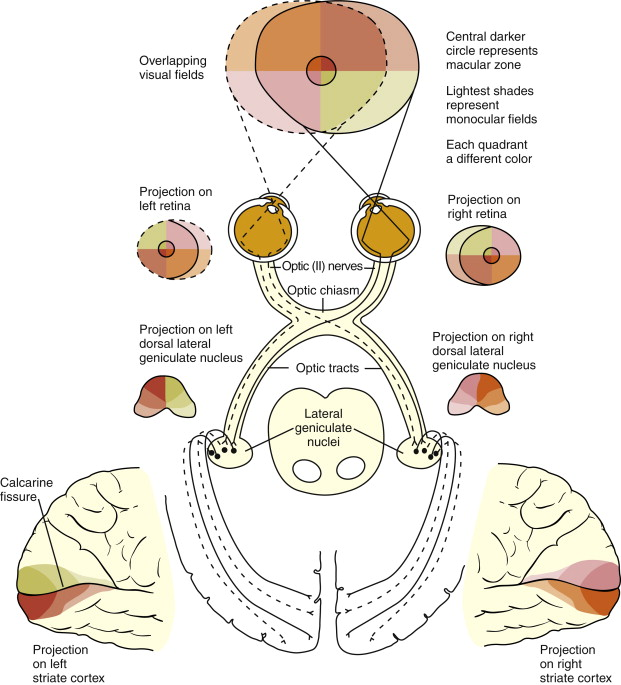
\includegraphics[width=325pt]{via_visual.jpg}
\caption{Vários componentes envolvidos no processamento de informação visual \cite{via_visual_primaria}.}
\label{fig:via_visual}
\end{figure}

\section{Redes Neuronais Convolucionais}
\label{chap2:sec:funcionamento}
Apresentada a estrutura biológica que inspirou o investimento nas Redes Neuronais artificiais, importa descrever os mecanismos que levam uma CNN a conseguir replicar (com as devidas diferenças) o processo anteriormente descrito. \newline

\noindent Tipicamente, uma CNN tem as seguintes camadas: camada(s) convolucional(ais), camada(s) de \textit{pooling} e camada(s) de classificação (camada(s) completamente ligada(s)).

\subsection{Camada Convolucional}
\label{chap2:subsec:convolucional}
Esta camada procura detetar \textit{features} de baixo nível, como arestas e curvas. Para tal, é usado um filtro (também chamado de \textit{kernel}). Uma imagem tem sempre a forma NxMxC, sendo N o número de linhas, M o número de colunas e C o número de canais de cor. De modo a diminuir o tamanho potencialmente inviável do \textit{input}, o \textit{kernel} (nada mais que uma matriz) passa pela imagem um número permitido de vezes - numa matriz 5x5 e com passo/\textit{stride} igual a 1, o \textit{kernel} cobre-a nove vezes originando um mapa de ativação 3x3 (figura \ref{fig:kernel}).


\noindent Note-se que outras etapas podem ser acrescentadas ao output da camada convolucional (por exemplo, a função de ativação ReLU promove não-linearidade, algo desejável quando se trabalha com imagens que não são lineares, por natureza) 

\begin{figure}[h]
\centering
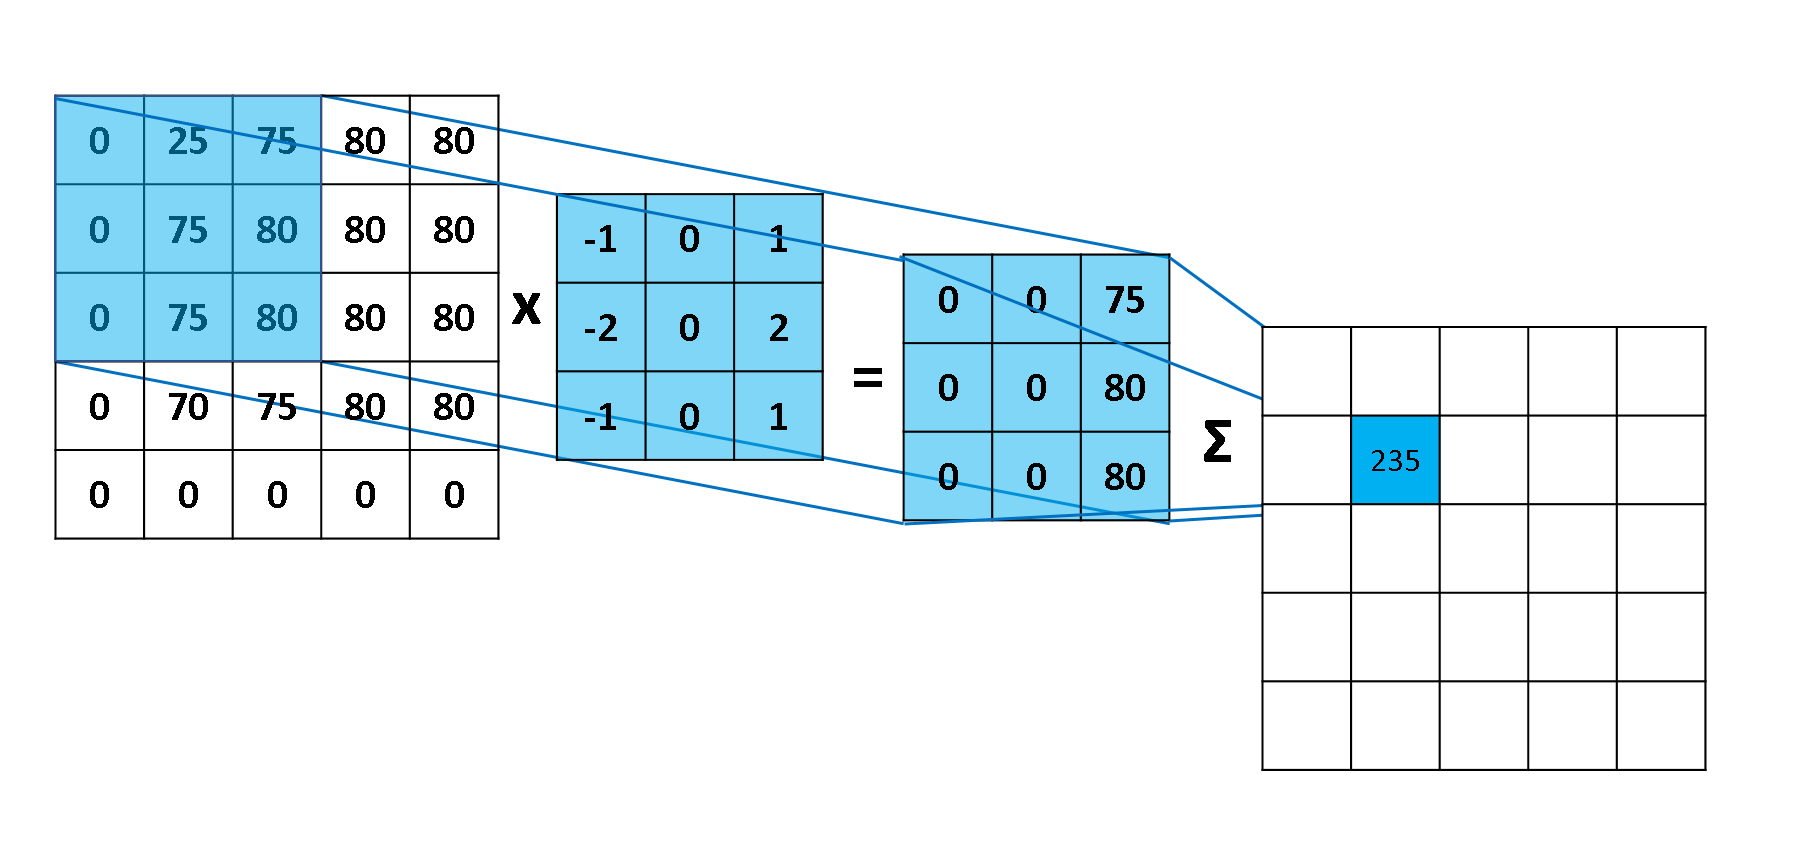
\includegraphics[width=350pt]{kernel.png}
\caption{Operação de convolução entre uma matriz de entrada 5x5 e um \textit{kernel} 3x3 \cite{kernel}.}
\label{fig:kernel}
\end{figure}

\noindent Os valores do \textit{kernel} são multiplicados com os da área abrangida na matriz inicial, sendo posteriormente somados (a matriz com todos estes números calculados contém as chamadas \textit{convolved features}).

\noindent O exemplo retratado na figura \ref{fig:kernel} representa uma simplificação do processo de convolução. Na realidade, podem-se considerar situações adicionais:

\begin{enumerate}
        \item No caso de uma imagem a cor RGB, existem três canais, pelo que a matriz de \textit{input} tem profundidade igual a 3. O \textit{kernel} é aplicada a cada canal e os três valores resultantes de cada canal são somados, dando, finalmente, o valor que entrará na matriz das \textit{convolved features}.
    \item De modo a extrair mais \textit{features}, podem ser utilizados vários \textit{kernels} com pesos diferentes. Assim, obtém-se um volume no fim desta camada, e não um \textit{output} com profundidade igual a 1.
\end{enumerate}

\subsection{Camada de \textit{Pooling}}
\label{chap2:subsec:pooling}
\noindent Sendo aplicada ao \textit{output} da etapa anterior, a camada de \textit{pooling} tem a função de reduzir a dimensão espacial das \textit{convolved features}, sem perder informação necessária à classificação. Esta camada é, ainda, capaz, de extrair \textit{features} dominantes em certas regiões da imagem de entrada. Consideram-se dois tipos de \textit{pooling}: \textit{max pooling} e \textit{average pooling}.\newline
\noindent A técnica de \textit{max pooling} opta por, a partir de uma região definida na matriz das \textit{convolved features}, escolher o maior valor possível (figura \ref{fig:pooling}). Apresenta a vantagem de reduzir possível ruído e combater o problema de \textit{overfitting} - manifesta-se quando os resultados no conjunto de teste são muito bons, mas a mesma \textit{performance} não se verifica nos exemplos de teste. \newline
\noindent Numa abordagem alternativa, \textit{average pooling} faz a média aritmética simples dos valores abrangidos pelo filtro escolhido, normalmente 2x2 e com passo/\textit{stride} semelhante (figura \ref{fig:pooling}). \newline
\noindent Comparando as duas variantes, \textit{max pooling} é a mais popular, sendo creditada como a melhor em termos de \textit{performance}.

\begin{figure}[h]
\centering
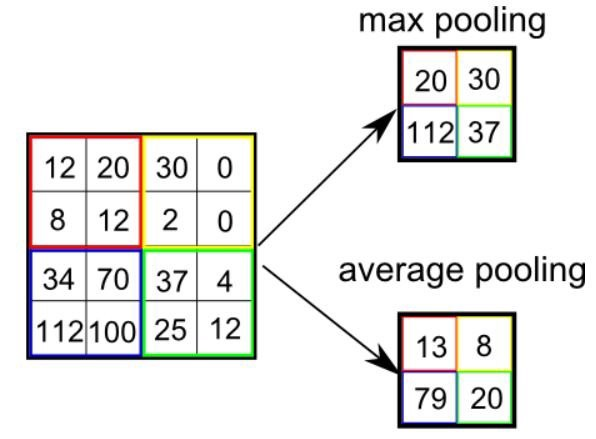
\includegraphics[width=185pt]{pooling.jpg}
\caption{2 tipos de \textit{pooling} \cite{pool}.}
\label{fig:pooling}
\end{figure}

\noindent Dependendo da aplicação e \textit{dataset} a analisar, podem ser usadas várias camadas convolucionais e de \textit{pooling} intercaladas.

\subsection{Camada Completamente Ligada}
\label{chap2:subsec:fully}
Em qualquer caso, o volume (matriz com profundidade) resultante da intercalação das camadas anteriormente mencionadas, será achatado na forma de um vetor coluna. Deste modo, é possível fornecer tal vetor, como \textit{input}, a uma rede neuronal tradicional (sendo que os neurónios de cada camada estão ligados com todos os da camada seguinte). Pode-se dizer que as camadas anteriores extraíram \textit{features} da imagem de entrada, enquanto que as camadas que se seguem classificam tudo o que foi obtido (dando mais importância a determinados padrões e formas que outros).

\noindent Na figura \ref{fig:fully}, os círculos amarelos representam o resultado da interpolação de "n" camadas de convolução e \textit{pooling}. Os círculos azuis agem como uma rede neuronal (tipicamente um \ac{MLP}) com tantas camadas escondidas quantas as necessárias para o problema a ser tratado. Finalmente, a última camada (vermelha), contém os neurónios ligados às classes existentes. É comum usar-se a função \textit{softmax} para obter uma distribuição probabilística sobre os \textit{outputs} finais da CNN.\newline

\begin{figure}[h]
\centering
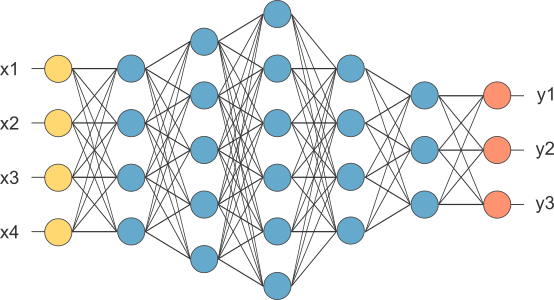
\includegraphics[width=330pt]{fully.png}
\caption{Visualização das camadas finais de uma CNN \cite{fully}.}
\label{fig:fully}
\end{figure}

\subsection{Função de \textit{Loss}}
\label{chap2:subsec:loss}
Uma função de \textit{loss} mede a performance de um modelo de classificação. No caso mais concreto dos problemas trabalhados, foi usada a função \textit{Cross-Entropy}. Apresenta a seguinte fórmula:

\begin{equation}
 H_{p}(q) = -\frac{1}{N}\sum_{i=1}^{N}y_{i}\log(p(y_{i}))+(1-y_{i})\log(1-p(y_{i}))
 \label{eq:eq_log}
\end{equation}

\noindent Na fórmula \ref{eq:eq_log}, \emph{$y_{i}$} representa a classe verdadeira de um dado ponto \emph{i}, N o número de pontos/elementos a classificar e \emph{$p(y_{i})$} a probabilidade de o ponto ser da classe 1. Numa análise à fórmula, se o ponto for da classe 1 (aplica-se em problemas binários, logo as classes são 1 e 0), o segundo termo anula-se e fica apenas \emph{$log(p(y_{i}))$}. Relembrando a curva logarítmica, uma probabilidade alta faria o termo ser próximo de 0 (aproximando-se pelos valores negativos). \newline 
\noindent De forma inversa, um ponto de classe 0 anula o primeiro termo e resulta em \emph{$log(1-p(y_{i}))$}. Como é de classe 0, a probabilidade de ser de classe 1 é, idealmente, baixa. Logo o valor dentro do logaritmo será próximo de 1 e a imagem respetiva, na função logarítmica, próxima de 0.\newline
\noindent Por fim, é invertido o valor resultante do somatório (os logaritmos de cada ponto resultaram em valores negativos) e feita a média das entropias cruzadas obtidas (\emph{$\frac{1}{N}$}).

\subsection{Notas finais}
\label{chap2:subsec:notas}
Nos últimos 20 anos, várias arquiteturas para \ac{CNN}s foram propostas, destacando-se as seguintes:

\begin{enumerate}
    \item \textbf{LeNet-5}, proposta por Yann LeCun em 1998, propunha-se a classificar dígitos, escritos à mão, digitalizados com uma resolução de 32x32 em escala de cinza.
    \item \textbf{AlexNet}, descrita por Alex Krizhevsky num \textit{paper} publicado em 2012, venceu a \ac{ILSVRC} do mesmo ano com uma vantagem de mais de 10\% para o segundo lugar. Conta com cinco camadas convolucionais (algumas seguidas de camadas de \textit{pooling}) e três camadas completamente ligadas. Propõe, ainda, o uso da função de ativação ReLU. Esta arquitetura demonstrou como a profundidade de uma rede é crucial para o desempenho final, bem como, técnicas de aumento de dados (espelhar ou cortar imagens) e de \textit{dropout} (remover neurónios aleatoriamente) ajudam a combater o problema de \textit{overfitting}.
    \item \textbf{GoogleNet/Inception}, vencedora da \ac{ILSVRC} de 2014 com um erro top-5 de 6.67\% (entrando no nível de performance do próprio ser humano). Conta com 22 camadas, vários módulos Inception (fazem várias convoluções e \textit{pooling}) e reduz o número de parâmetros da AlexNet (60 milhões) para apenas 4 milhões.
    \item \textbf{VGGNet}, perdeu em 2014 para a GoogleNet, sendo creditada pela capacidade de extração de \textit{features}. Como desvantagem, contém 138 milhões de parâmetros.
    \item \textbf{ResNet}, vencedora da  \ac{ILSVRC} de 2015, possui 152 camadas. Note-se que, mesmo assim, possui menor complexidade que a VGG.
\end{enumerate}

\noindent Devido à reconhecida capacidade de classificação de imagens, foi usada uma \ac{CNN} (mais concretamente, a arquitetura Inception) com vista a solucionar os dois problemas descritos nos capítulos seguintes.
\clearpage{\thispagestyle{empty}\cleardoublepage}
\chapter{Problema 1: Validação de Módulo de Tracking}
\label{chap:val_ids}

\section{Introdução}
\label{chap3:sec:intro}
Durante um processo de \textit{tracking} de qualquer objeto, erros podem acontecer. No caso específico abordado pelo presente projeto, a partir de imagens captadas por painéis de \textit{outdoor}, \textit{bounding boxes} foram colocadas ao redor das pessoas que passavam pelos locais abrangidos. IDs únicos foram igualmente atribuídos, constituindo, em teoria, a ação de \textit{tracking}.

\noindent Assim, o primeiro desafio proposto passou por validar os IDs atribuídos aos diferentes indivíduos, tomando como entrada uma sequência de \textit{patches} e avaliar se diz respeito ao  mesmo indivíduos ou a indivíduos diferentes.

\begin{figure} [h]
  \centering
  \begin{subfigure}{385pt}
    \centering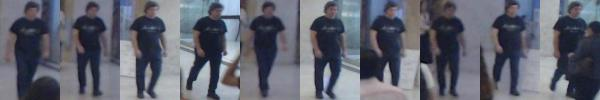
\includegraphics[width=385pt]{capa.jpg}
    \caption{}
  \end{subfigure}
  \begin{subfigure}{385pt}
    \centering
\includegraphics[width=385pt]{capa2.jpg}
    \caption{}
  \end{subfigure}
  \caption{Exemplos de sequências respeitantes a um mesmo indivíduo (a) e a indivíduos diferentes (b).}
  \label{fig:imagem_exemplo}
\end{figure}

\section{Pré-processamento dos dados}
\label{chap3:sec:metodo}
Antes de passarem pela etapa de aprendizagem, os dados foram trabalhados de modo a configurarem entradas válidas na \ac{CNN}. A figura \ref{fig:movimentos} apresenta alguns casos práticos e a figura 3.3 apresenta de forma esquemática as etapas necessárias, sendo expostas com maior detalhe nas secções seguintes. \newline

\begin{figure} [h]
  \centering
  \begin{subfigure}{4cm}
    \centering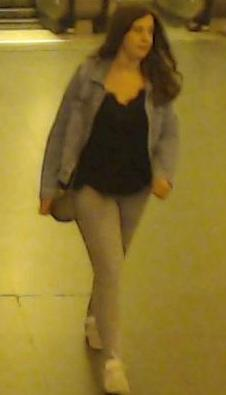
\includegraphics[width=3.5cm]{aproxima.jpg}
    \caption{}
  \end{subfigure}
  \begin{subfigure}{4cm}
    \centering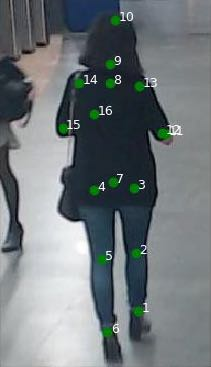
\includegraphics[width=3.5cm]{esqueleto.jpg}
    \caption{}
  \end{subfigure}
  \begin{subfigure}{4cm}
    \centering
\includegraphics[width=3.5cm]{lateral.jpg}
    \caption{}
  \end{subfigure}
  \caption{3 principais tipos de movimento: aproximação (a), afastamento - com dados de pose - (b) e lateral (c).}
  \label{fig:movimentos}
\end{figure}

\begin{figure}[h]
    \centering
    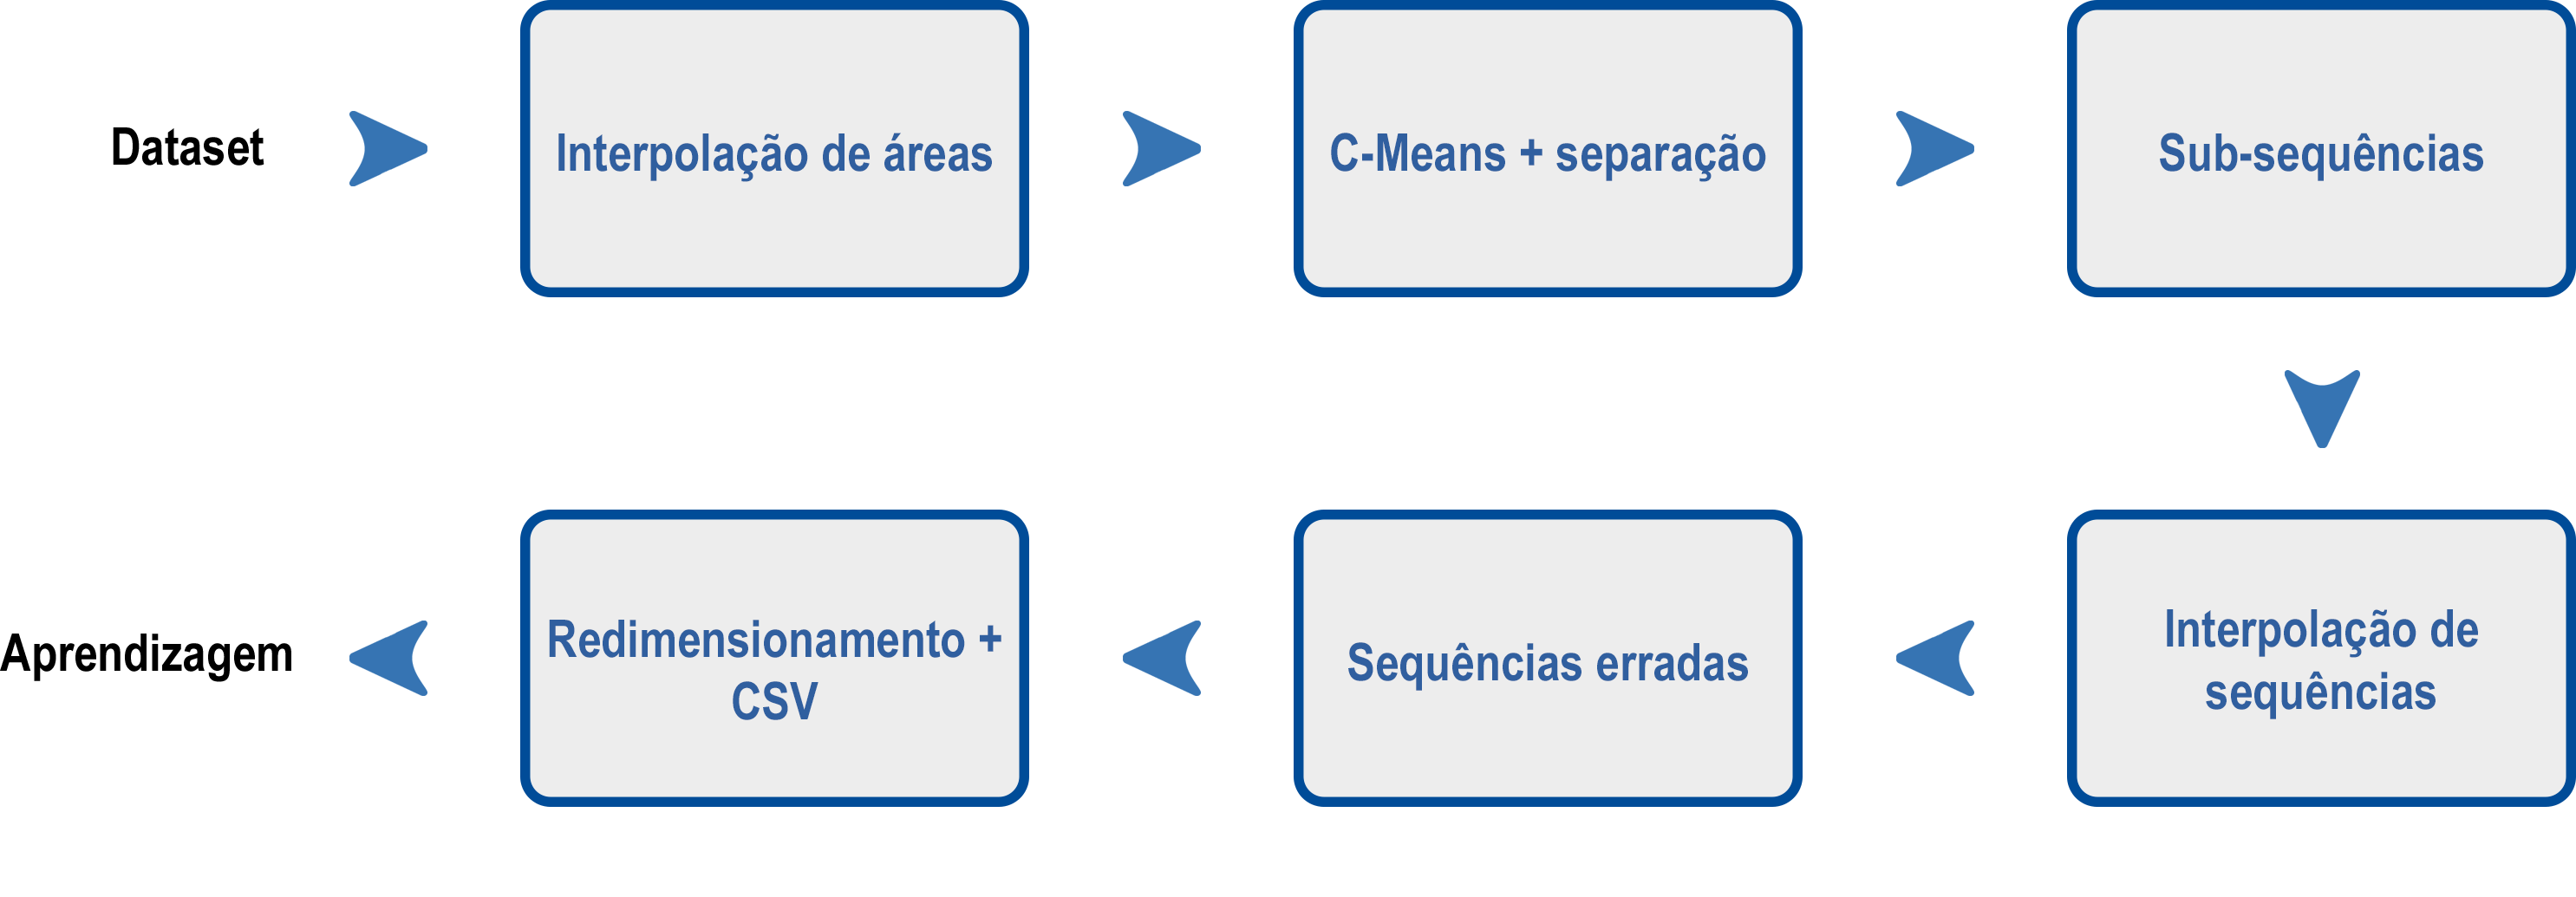
\includegraphics[width=380pt]{pipeline.png}
    \label{fig:pipeline}
    \caption{\textit{Pipeline} de pré-processamento.}
    \end{figure}

\subsection{Interpolação de áreas}
\label{chap3:subsec:areas}
Cada \textit{patch} de cada indivíduo possui, naturalmente, uma altura e uma largura (em píxeis), e, por consequência, uma área. Numa primeira fase é importante discriminar o tipo de movimento de uma pessoa para a geração de instâncias erradas de uma sequência ser possível (mais se acrescenta num próximo ponto). Assim, as áreas são calculadas, normalizadas no intervalo [0,1] e interpoladas (para haver um número constante para todos os indivíduos). 

\noindent Note-se que existe a possibilidade de existirem menos \textit{patches} do que o número definido (25, por exemplo). A solução passou por obter o gráfico do movimento com os dados reais e calcular dados artificiais. A figura 3.4 apresenta um movimento de afastamento expandido.
    
\begin{figure}[h]
\centering
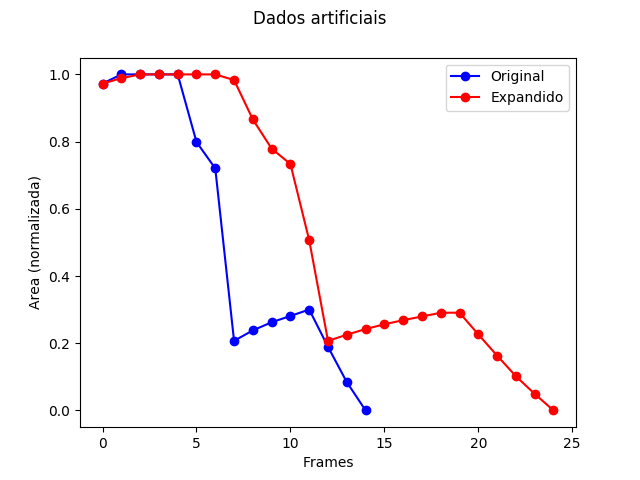
\includegraphics[width=270pt]{interpolada.png}
\label{fig:dados_artificiais_foto}
\caption{Obtenção de mais valores de área.}
\end{figure}

\subsection{Algoritmo C-Means e separação de sequências}
\label{chap3:subsec:cmeans}
O algoritmo C-Means representa uma forma de \textit{fuzzy clustering}, na qual os elementos são agrupados em \textit{clusters} de acordo com as suas caraterísticas. Elementos de um mesmo \textit{cluster} tendem a ser o mais semelhantes possível, enquanto que se procura maximizar a diferença entre elementos de \textit{clusters} distintos. De notar que um elemento pode pertencer a um ou mais \textit{clusters}.

\noindent A noção de pertença (ou \textit{membership}) é basilar neste algoritmo. Pontos/elementos mais afastado do centro de um \textit{cluster} têm graus de \textit{membership} mais baixos; em sentido inverso, quanto mais perto do centro, maior é o grau. 

\noindent O propósito deste algoritmo passa por minimizar a seguinte função objetivo:

\begin{equation}
 \operatorname*{argmin}_C\sum_{i=1}^{C}\sum_{k=1}^{N}u_{ik}^m||x_k-c_i||^2.
 \label{eq:eq1}
\end{equation}

\noindent Na fórmula \ref{eq:eq1} o parâmetro \emph{C} representa o número de grupos a considerar, \emph{N} o número de pontos/elementos, \emph{m} o \textit{fuzzifier} (tem efeito sobre a performance do algoritmo) e \emph{$u_{ik}$} o coeficiente de \textit{membership} (aparece multiplicado pela distância de cada ponto - \emph{$x_k$} - a um dado centro - \emph{$c_i$}). Por sua vez, os coeficientes de \textit{membership} e os centros possuem as seguintes fórmulas, respetivamente:

\begin{equation}
u_{ik} = \frac{1}{\sum_{j=1}^{C}{\left( \frac{||x_k-c_i||^2}{||x_k-c_j||^2} \right)}^{\left( \frac{1}{m-1}\right)}}.
 \label{eq:eq2}
\end{equation}

\begin{equation}
c_{i} = \frac{\sum_{k=1}^{N}{u_{ik}^{m}x_k}}{\sum_{k=1}^{N}{u_{ik}^{m}}}.
 \label{eq:eq3}
\end{equation}

\noindent A execução do algoritmo baseia-se em em várias iterações com vista a minimizar a função objetivo (\ref{eq:eq1}) e cujo critério de paragem é, normalmente, atingido quando a diferença entre os coeficientes obtidos em iterações sucessivas for menor que um dado parâmetro (\emph{$\epsilon$}).

\noindent O C-Means foi aplicado sobre os valores normalizados e interpolados das áreas, para obter os dois padrões dominantes (essencialmente, os movimentos de afastamento e aproximação) - figura 3.5. Os valores de cada indivíduo são depois comparados com cada padrão, determinando com qual dos dois existe maior semelhança. Adicionalmente, os dados de pose (fornecidos com este \textit{dataset}) são também usados para determinar o tipo de movimento, nomeadamente através da posição dos ombros entre si.

\begin{figure}[h]
\centering
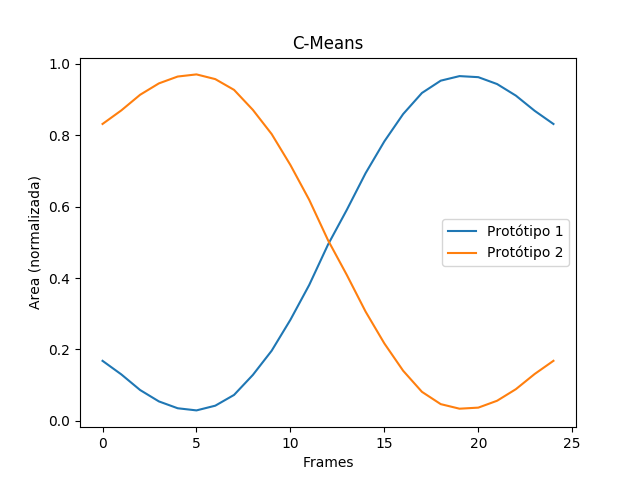
\includegraphics[width=220pt]{c-means_25.png}
\label{fig:c_means}
\caption{Padrões extraídos com o C-Means.}
\end{figure}

\subsection{Geração de sub-sequências}
\label{chap3:subsec:sub}
De modo a aumentar a quantidade de dados disponíveis, foram geradas sub-sequências a partir das sequências separadas anteriormente. Uma sub-sequência é simplesmente uma variação da original. Por exemplo, a partir de uma sequência com 20 \textit{patches}, pode-se obter uma variação que contém as imagens no intervalo [1,15].

\subsection{Interpolação de sequências}
\label{chap3:subsec:interpolar_seq}
Dado que nem todos os indivíduos têm o mesmo número de \textit{patches}, definiu-se um tamanho constante para as sequências dadas à \ac{CNN}. Todas as sequências que não cumprirem com este requisito são descartadas. Por outro lado, se uma sequência tiver mais imagens que as necessárias, será interpolada para atingir o tamanho desejado.

\subsection{Geração de sequências erradas}
\label{chap3:subsec:erradas}
Para cada sequência foi gerada uma instância errada. Se o tamanho definido para as sequências for "x", "x-1" ou "x-2" imagens mantêm-se na sequência errada. No caso de só se trocar uma imagem, a que não se manteve é substituída por uma de outra sequência (efetivamente outro indivíduo do mesmo conjunto - treino, validacao ou teste - com um tipo de movimento semelhante). O processo é semelhante se se trocarem duas imagens. Esta troca pode ser feita de forma aleatória ou de forma mais informada (e difícil de detetar):

\begin{enumerate}
    \item \textbf{Troca aleatória:} É sorteado um indivíduo do mesmo conjunto. Uma ou duas \textit{patches} são colocadas na instância errada da sequência original, completando a errada.
    \item \textbf{Troca informada:} É escolhido o indivíduo mais aproximado ao da sequência original, sendo que todos os indivíduos candidatos são classificados num total de 100 pontos - 80 dizem respeito à cor da roupa e 20 às \textit{soft biometrics} dos indivíduos, como o tipo e cor de cabelo, a fisionomia do corpo, entre outros. \newline \noindent O indivíduo com menor distância em termos de cor em cada um dos 16 pontos de esqueleto recebe 80 pontos; o segundo melhor recebe um pouco menos e assim sucessivamente (com os extras o processo é análogo). Note-se que a distância de cor para cada ponto de esqueleto é a distância entre as três cores RGB dos pontos.\newline \noindent Estando escolhido o indivíduo com melhor classificação, são colocadas as \textit{patches} na instância errada a ser construída num dado momento. 
\end{enumerate}{}

\begin{figure} [h]
  \centering
  \begin{subfigure}{13.5cm}
    \centering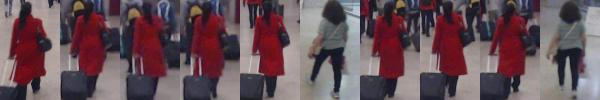
\includegraphics[width=13.5cm]{troca_aleatoria.jpg}
    \caption{}
  \end{subfigure}
  \begin{subfigure}{13.5cm}
    \centering
\includegraphics[width=13.5cm]{troca_boa.jpg}
    \caption{}
  \end{subfigure}
  \caption{Troca aleatória (a) e informada (b).}
  \label{fig:trocas}
\end{figure}

\subsection{Redimensionamento das sequências e ficheiro CSV}
\label{chap3:subsec:redim}
A \ac{CNN} usada requer que todas as imagens de entrada tenham um tamanho constante. Assim esta etapa passa por redimensionar todas as \textit{patches} para um tamanho único (definiu-se 60x100).\newline
\noindent Por último, é gerado um ficheiro CSV em que cada linha representa uma sequência, sendo marcadas como destinadas a treino, validação ou teste, bem como se são certas (sempre o mesmo indivíduo) ou erradas. \newline
\noindent

\section{Fase de aprendizagem}
\label{chap3:sec:aprendizagem}
O processo de treino da \ac{CNN} possui variabilidade, nomeadamente na geração de instâncias erradas para cada sequência válida. Tais variações têm impacto na performance sobre os conjuntos de treino, validação e, sobretudo, de teste.\newline
\noindent A figura \ref{fig:graficos} apresenta várias instâncias de aprendizagem, cujas diferenças residem na variablidade acima mencionada.

\noindent Na figura \ref{fig:graficos} estão as seguintes configurações:
\begin{enumerate}[(a)]
    \item Treino e validação informados + teste informado.
    \item Treino e validação informados + teste aleatório.
    \item Treino e validação aleatórios + teste informado.
    \item Treino e validação aleatórios + teste aleatório.
\end{enumerate}{}

\begin{figure} [h]
  \centering
  \begin{subfigure}{6.8cm}
    \centering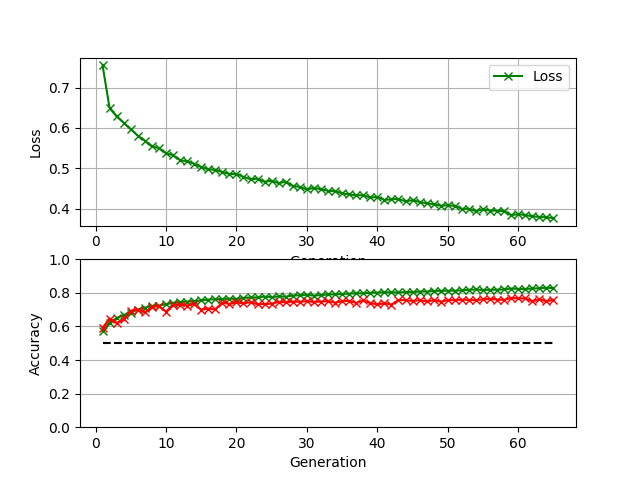
\includegraphics[width=6.8cm]{bom_bom.png}
    \caption{}
  \end{subfigure}
  \begin{subfigure}{6.8cm}
    \centering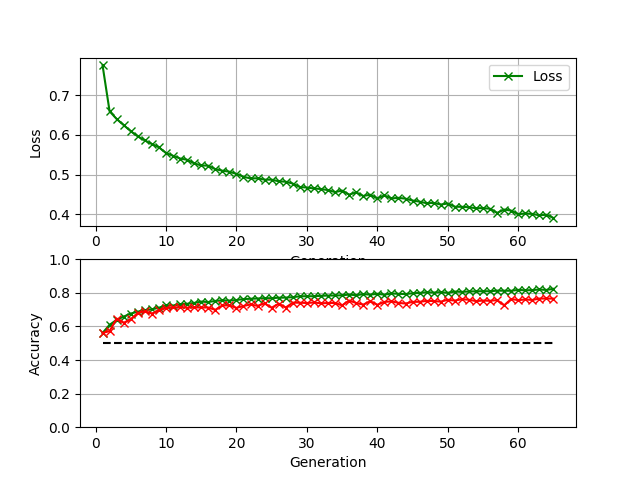
\includegraphics[width=6.8cm]{bom_mau.png}
    \caption{}
  \end{subfigure}
  \begin{subfigure}{6.8cm}
    \centering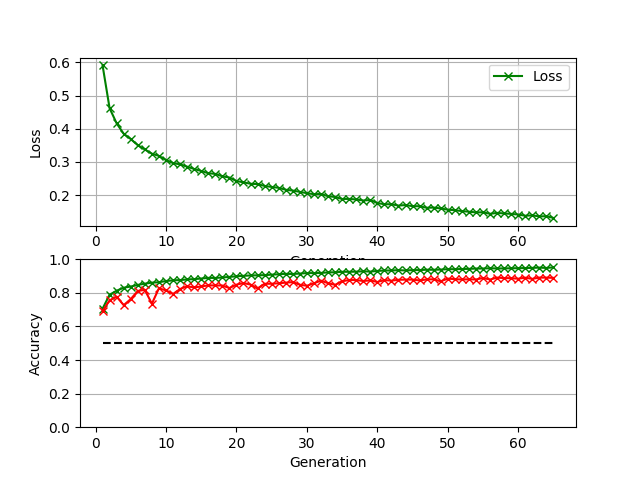
\includegraphics[width=6.8cm]{mau_bom.png}
    \caption{}
  \end{subfigure}
  \begin{subfigure}{6.8cm}
    \centering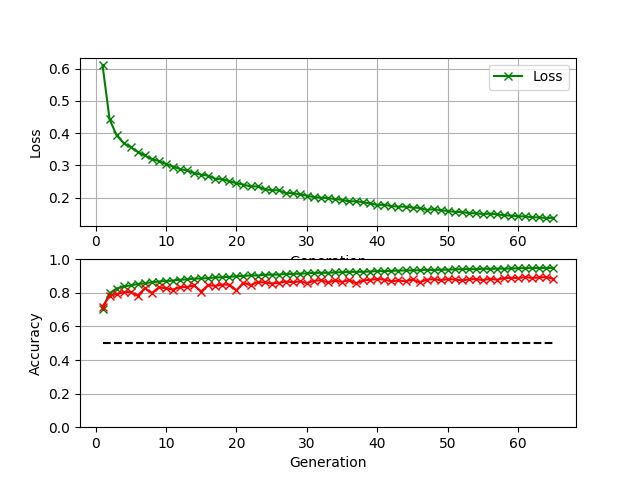
\includegraphics[width=6.8cm]{mau_mau.png}
    \caption{}
  \end{subfigure}
  \caption{Resultados da aprendizagem com 4 configurações diferentes.}
  \label{fig:graficos}
\end{figure}

\begin{table} [!htbp]
\centering
\begin{tabular}{|l|r|r|}
\hline
\textbf{Configuração} & \textbf{Sequências} & \textbf{Acerto}\\
\hline
\hline
Treino e validação informados + teste informado & $\sim62000$ & 78\% \\
\hline
Treino e validação informados + teste aleatório & $\sim63000$ & 84\% \\
\hline
Treino e validação aleatórios + teste informado & $\sim112000$ & 78\% \\
\hline
Treino e validação aleatórios + teste aleatório & $\sim111000$ & 90\% \\
\hline
\end{tabular}
\caption{Taxa de acerto sobre diferentes configurações.}
\label{tab:resultados}
\end{table}

\noindent A tabela \ref{tab:resultados} mostra que se a rede for treinada com um conjunto fácil, existe uma diferença mais significativa entre a performance com dados de teste mais fáceis e mais difíceis (de quase 90\% passa para 78\%). Em contraste, com um treino mais difícil a diferença revela-se muito menor (de quase 84\% para 78\%).


\noindent Note-se que as configurações c) e d) têm mais dados de entrada devido ao facto de que para construir as instâncias negativas de forma informada são usados os dados de pose, sendo que nem todas as imagens os têm.

\section{Discussão e Resultados}
\label{chap3:sec:final}
Uma análise às sequências analisadas pela rede revela alguns casos típicos de falha: uma troca feita na sequência e que a rede não foi capaz de detetar; uma sequência certa mas que contém uma ou mais \textit{patches} com certo ruído (partes de outras pessoas) ou uma sequência com muita interferência (figura \ref{fig:falha}).

\begin{figure} [h]
  \centering
  \begin{subfigure}{13.5cm}
    \centering
\includegraphics[width=13.5cm]{erro_troca_boa.jpg}
    \caption{}
  \end{subfigure}
  \begin{subfigure}{13.5cm}
    \centering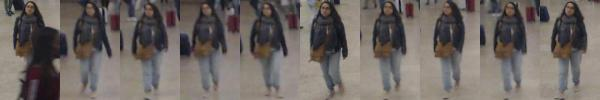
\includegraphics[width=13.5cm]{erro_peq_ruido.jpg}
    \caption{}
  \end{subfigure}
  \begin{subfigure}{13.5cm}
    \centering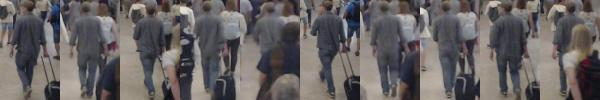
\includegraphics[width=13.5cm]{erro_grande_ruido.jpg}
    \caption{}
  \end{subfigure}
  \caption{Casos típicos de falha.}
  \label{fig:falha}
\end{figure}

\noindent O programa desenvolvido tem como objetivo tomar como entrada uma sequência de tamanho e dimensões iguais aos usados na aprendizagem, e devolver uma simples frase, consoante a sequência diz respeito ao mesmo indivíduo ou a indivíduos diferentes.\newline
\noindent Para testar a solução desenvolvida foram separadas 50 sequências (nunca vistas pela rede) recolhidas de diferentes painéis e em condições de luminosidade diversas, sendo 25 positivas e 25 negativas.\newline
\noindent A taxa de acerto foi de cerca de 52\% usando tanto o modelo treinado com os conjuntos de treino, validação e teste construídos usando a troca informada como usando a troca aleatória. Os parâmetros usados estão descritos na seguinte tabela:

\begin{table}[H]
\centering
\begin{tabular}{|l|r|}
\hline
\textbf{Parâmetro} & \textbf{Valor}\\
\hline
\hline
Épocas & 65  \\
\hline
Taxa de aprendizagem & 0.001  \\
\hline
Probabilidade de \textit{dropout} & 1.0  \\
\hline
Tamanho de \textit{batch} & 100  \\
\hline
Sequências & $\sim75000$  \\
\hline
\hline
\textbf{Acerto (conj. teste)} & \textbf{52\%}\\
\hline
\end{tabular}
\caption{Parâmetros base.}
\label{tab:base}
\end{table}

\noindent Alguns parâmetros foram alterados com vista a avaliar o impacto na performance do sistema. O conjunto de teste usado foi formado pelas 100 sequências separadas (também usadas na performance base, anteriormente descrita). As tabelas seguintes apresentam os parâmetros alterados:

\begin{table}[H]
\centering
\begin{tabular}{|l|r|}
\hline
\textbf{Parâmetro} & \textbf{Valor}\\
\hline
\hline
Épocas & 65  \\
\hline
\textbf{Taxa de aprendizagem} & \textbf{0.0001}  \\
\hline
Probabilidade de \textit{dropout} & 1.0  \\
\hline
Tamanho de \textit{batch} & 100  \\
\hline
Sequências & $\sim75000$  \\
\hline
\hline
\textbf{Acerto (conj. teste)} & \textbf{51\%}\\
\hline
\end{tabular}
\caption{Mudança na taxa de aprendizagem.}
\label{tab:learning_rate}
\end{table}

\begin{table}[H]
\centering
\begin{tabular}{|l|r|}
\hline
\textbf{Parâmetro} & \textbf{Valor}\\
\hline
\hline
Épocas & 65  \\
\hline
Taxa de aprendizagem & 0.001  \\
\hline
\textbf{Probabilidade de \textit{dropout}} & \textbf{0.65}  \\
\hline
Tamanho de \textit{batch} & 100  \\
\hline
Sequências & $\sim75000$  \\
\hline
\hline
\textbf{Acerto (conj. teste)} & \textbf{56\%}\\
\hline
\end{tabular}
\caption{Mudança na probabilidade de \textit{dropout}.}
\label{tab:dropout}
\end{table}

\begin{table}[H]
\centering
\begin{tabular}{|l|r|}
\hline
\textbf{Parâmetro} & \textbf{Valor}\\
\hline
\hline
Épocas & 65  \\
\hline
Taxa de aprendizagem & 0.001  \\
\hline
Probabilidade de \textit{dropout} & 1.0  \\
\hline
\textbf{Tamanho de \textit{batch}} & \textbf{150}  \\
\hline
Sequências & $\sim75000$  \\
\hline
\hline
\textbf{Acerto (conj. teste)} & \textbf{54\%}\\
\hline
\end{tabular}
\caption{Mudança no tamanho de \textit{batch}.}
\label{tab:size}
\end{table}

\noindent Neste caso específico e dados os testes efetuados, o parâmetros que potencialmente afeta mais a performance da rede é a probabilidade de \textit{dropout}.
\clearpage{\thispagestyle{empty}\cleardoublepage}
\chapter{Problema 2: Identificação de Indivíduos}
\label{chap:ident_individuos}

\section{Introdução}
\label{chap4:sec:intro}
O reconhecimento facial de indivíduos, face a um \textit{dataset} conhecido, configurou o segundo desafio proposto. Foi usado o \textit{dataset} AR \cite{ar_site}, que contém 134 pessoas e mais de 3000 imagens (todas as pessoas têm imagens com diferente iluminação, expressões distintas ou adereços físicos). Alguns indivíduos registaram, ainda, imagens em dois dias diferentes (as mesmas variações acima mencionadas, mas registadas em dias distintos).


\noindent A figura \ref{fig:ar_dataset} apresenta as imagens recolhidas de um indivíduo, a título de exemplo.

\begin{figure}[h]
\centering
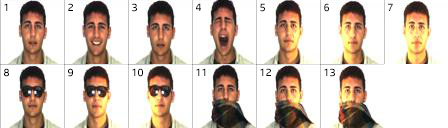
\includegraphics[width=380pt]{ar_dataset.png}
\caption{Exemplos de imagens do \textit{dataset} AR.}
\label{fig:ar_dataset}
\end{figure}
\newline
\noindent
\newline
\noindent
\newline
\noindent
\section{Pré-processamento dos dados}
\label{chap3:sec:metodo}
Ao contrário do processo descrito no capítulo anterior, as imagens deste \textit{dataset} já têm todas o mesmo tamanho e não existe necessidade de avaliar o tipo de movimento. Assim, apenas é necessário separá-las por indivíduo, gerar instâncias erradas para cada positiva e gerar o ficheiro CSV final (figura \ref{fig:processo2}).

\begin{figure}[h]
\centering

\includegraphics[width=380pt]{pipeline2.png}
\caption{\textit{Pipeline} de pré-processamento.}
\label{fig:processo2}
\end{figure}

\subsection{Separação das sequências}
\label{chap4:subsec:separacao}
Todas as imagens foram agrupadas de acordo com o indivíduo a que pertencem, sendo estes posteriormente divididos em conjuntos de treino, validação e teste (com a seguinte distribuição: 80\%, 10\% e 10\%).

\subsection{Geração de sequências erradas}
\label{chap4:subsec:erradas}

Foram exploradas duas formas de combinar as imagens dos indivíduos:

\begin{enumerate}
    \item \textbf{Sequências de duas imagens:} uma sequência certa será composta por duas imagens do mesmo indivíduo. Independentemente das caraterísticas específicas das imagens, se a pessoa for a mesma, a sequência é válida. \newline
    \noindent Para gerar sequências erradas, parte-se da sequência certa correspondente e é sorteado um outro indivíduo do mesmo conjunto (treino, validação ou teste) e uma das duas imagens, que se vai trocar pela equivalente do indivíduo sorteado. Por exemplo, se uma instância positiva tiver uma imagem em que o indíviduo sorri e outra em que está de óculos de sol, e for sorteada a dos óculos de sol, esta será substituída na instância errada pela imagem do indivíduo sorteado na qual também tem óculos de sol (figura \ref{fig:trocas2}).

    \begin{figure}[h]
      \centering
      \begin{subfigure}{3.6cm}
        \centering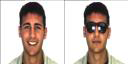
\includegraphics[width=3.6cm]{seq_certa.png}
        \caption{}
      \end{subfigure}
      \hspace{1em}
      \begin{subfigure}{3.6cm}
        \centering
\includegraphics[width=3.6cm]{seq_errada.png}
        \caption{}
      \end{subfigure}
      \caption{Sequência de duas imagens válida (a) e inválida (b).}
      \label{fig:trocas2}
    \end{figure}
    
    \item \textbf{Sequências de três imagens:} uma sequência certa será composta por duas imagens do mesmo indivíduo e uma imagem de outro indivíduo do mesmo conjunto. Deste modo, é possível obter mais combinações, não só para a aprendizagem mas também para a futura identificação de imagens nunca vistas.\newline
    \noindent Uma instância negativa consiste em manter duas imagens da positiva (uma das duas imagens do mesmo indivíduo e a do indivíduo diferente) e trocar a restante por uma equivalente (figura \ref{fig:trocas3}).
    
    \begin{figure}[h]
      \centering
      \begin{subfigure}{5.3cm}
        \centering
\includegraphics[width=5.3cm]{sequencia_3_boa.png}
        \caption{}
      \end{subfigure}
      \hspace{1em}
      \begin{subfigure}{5.3cm}
        \centering
\includegraphics[width=5.3cm]{sequencia_3_ma.png}
        \caption{}
      \end{subfigure}
      \caption{Sequência de três imagens válida (a) e inválida (b).}
      \label{fig:trocas3}
    \end{figure}
    
\end{enumerate}

\noindent Os conjuntos de imagens válidos e inválidos foram colocados num ficheiro .csv, necessário para a aprendizagem por parte da \ac{CNN}.

\section{Fase de aprendizagem}
\label{chap4:sec:aprendizagem}
A aprendizagem decorreu de acordo com os parâmetros e configurações descritos na tabela \ref{tab:aprendizagem_ar}, que contém também a taxa de acerto no conjunto de teste (os resultados são semelhantes nesta fase, quer seja com sequências de duas ou três imagens).

\begin{table}[h]
\centering
\begin{tabular}{|l|r|}
\hline
\textbf{Parâmetro} & \textbf{Valor}\\
\hline
\hline
Épocas & 65  \\
\hline
Probabilidade de \textit{dropout} & 1.0  \\
\hline
Tamanho de \textit{batch} & 100  \\
\hline
Sequências & $\sim75000$  \\
\hline
\hline
\textbf{Acerto (conj. teste)} & \textbf{82\%-83\%}\\
\hline
\end{tabular}
\caption{Parâmetros e configurações na aprendizagem.}
\label{tab:aprendizagem_ar}
\end{table}

\begin{figure}[h]
\centering
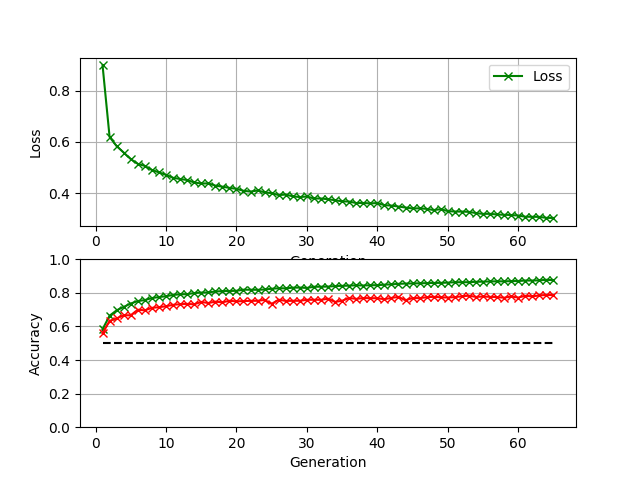
\includegraphics[width=300pt]{aprendizagem_ar.png}
\caption{Aprendizagem da \ac{CNN} sobre o \textit{dataset} AR.}
\label{fig:aprendizagem_dataset}
\end{figure}

\newline
\noindent
\newline
\noindent

\section{Discussão e Resultados}
\label{chap4:sec:final}
Foram desenvolvidos dois programas, usando os dois modelos treinados ora com duas sequências (chamado Face\_match1) ora com três (Face\_match2), cujo objetivo seria tomar como \textit{input} uma imagem nunca antes vista (colocada numa pasta específica) e retornar um ranking dos indivíduos com maiores chances de serem o indivíduo presente na foto de entrada.\newline
\noindent A título experimental, foi retirada, de cada pessoa, a imagem em que está zangada. Todas estas imagens foram então colocadas numa pasta própria e qualquer uma delas pode ser usada para testar o sistema desenvolvido. \newline

\noindent Para testar os dois sistemas desenvolvidos, foi usada uma galeria de imagens conhecidas pela rede (neste caso, as imagens de cada indivíduo com expressão neutra). 

\begin{figure}[h]
\centering

\includegraphics[width=350pt]{exemplo.png}
\caption{Objetivo dos sistemas desenvolvidos.}
\label{fig:exemplo}
\end{figure} 
\newline
\noindent A figura \ref{fig:face_match_rankings} apresenta algumas observações retiradas das experiências realizadas com as imagens passíveis de ser testadas (134 imagens com expressão zangada). 
\begin{figure}[H]
  \begin{subfigure}{15.0cm}
    \centering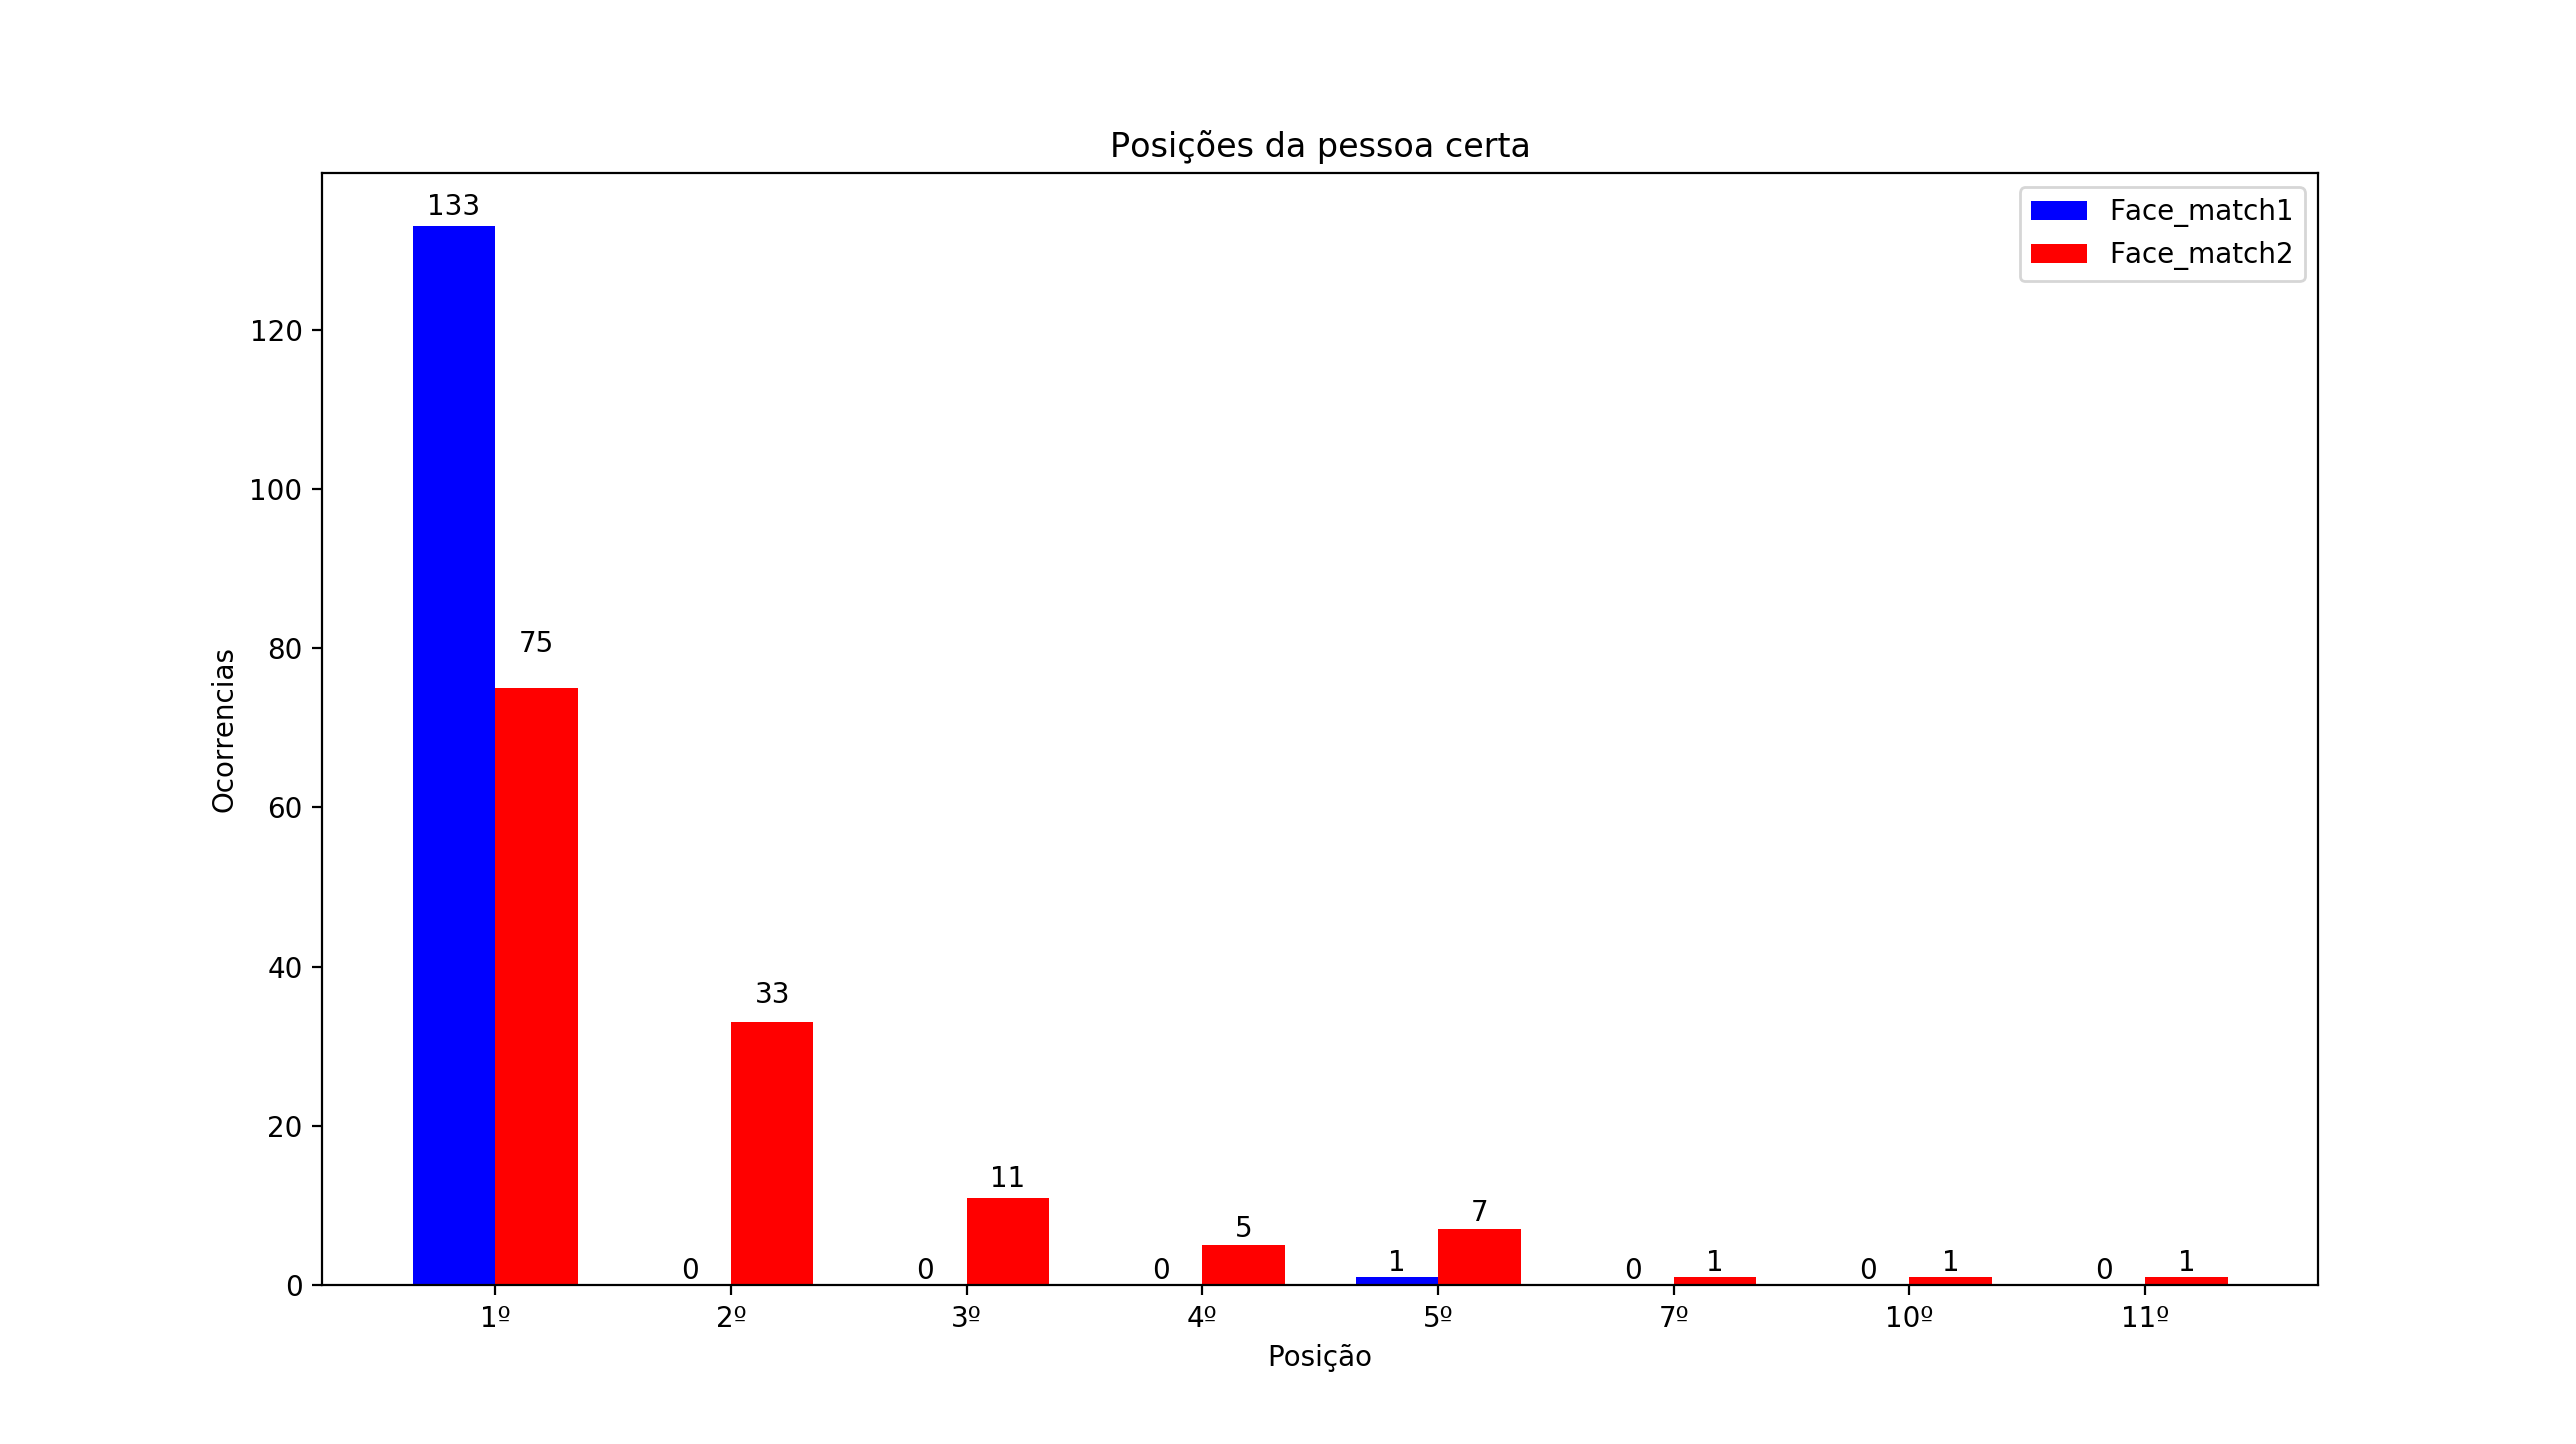
\includegraphics[width=15.0cm]{face_match_rankings.png}
    \caption{}
  \end{subfigure}
  \begin{subfigure}{15.0cm}
    \centering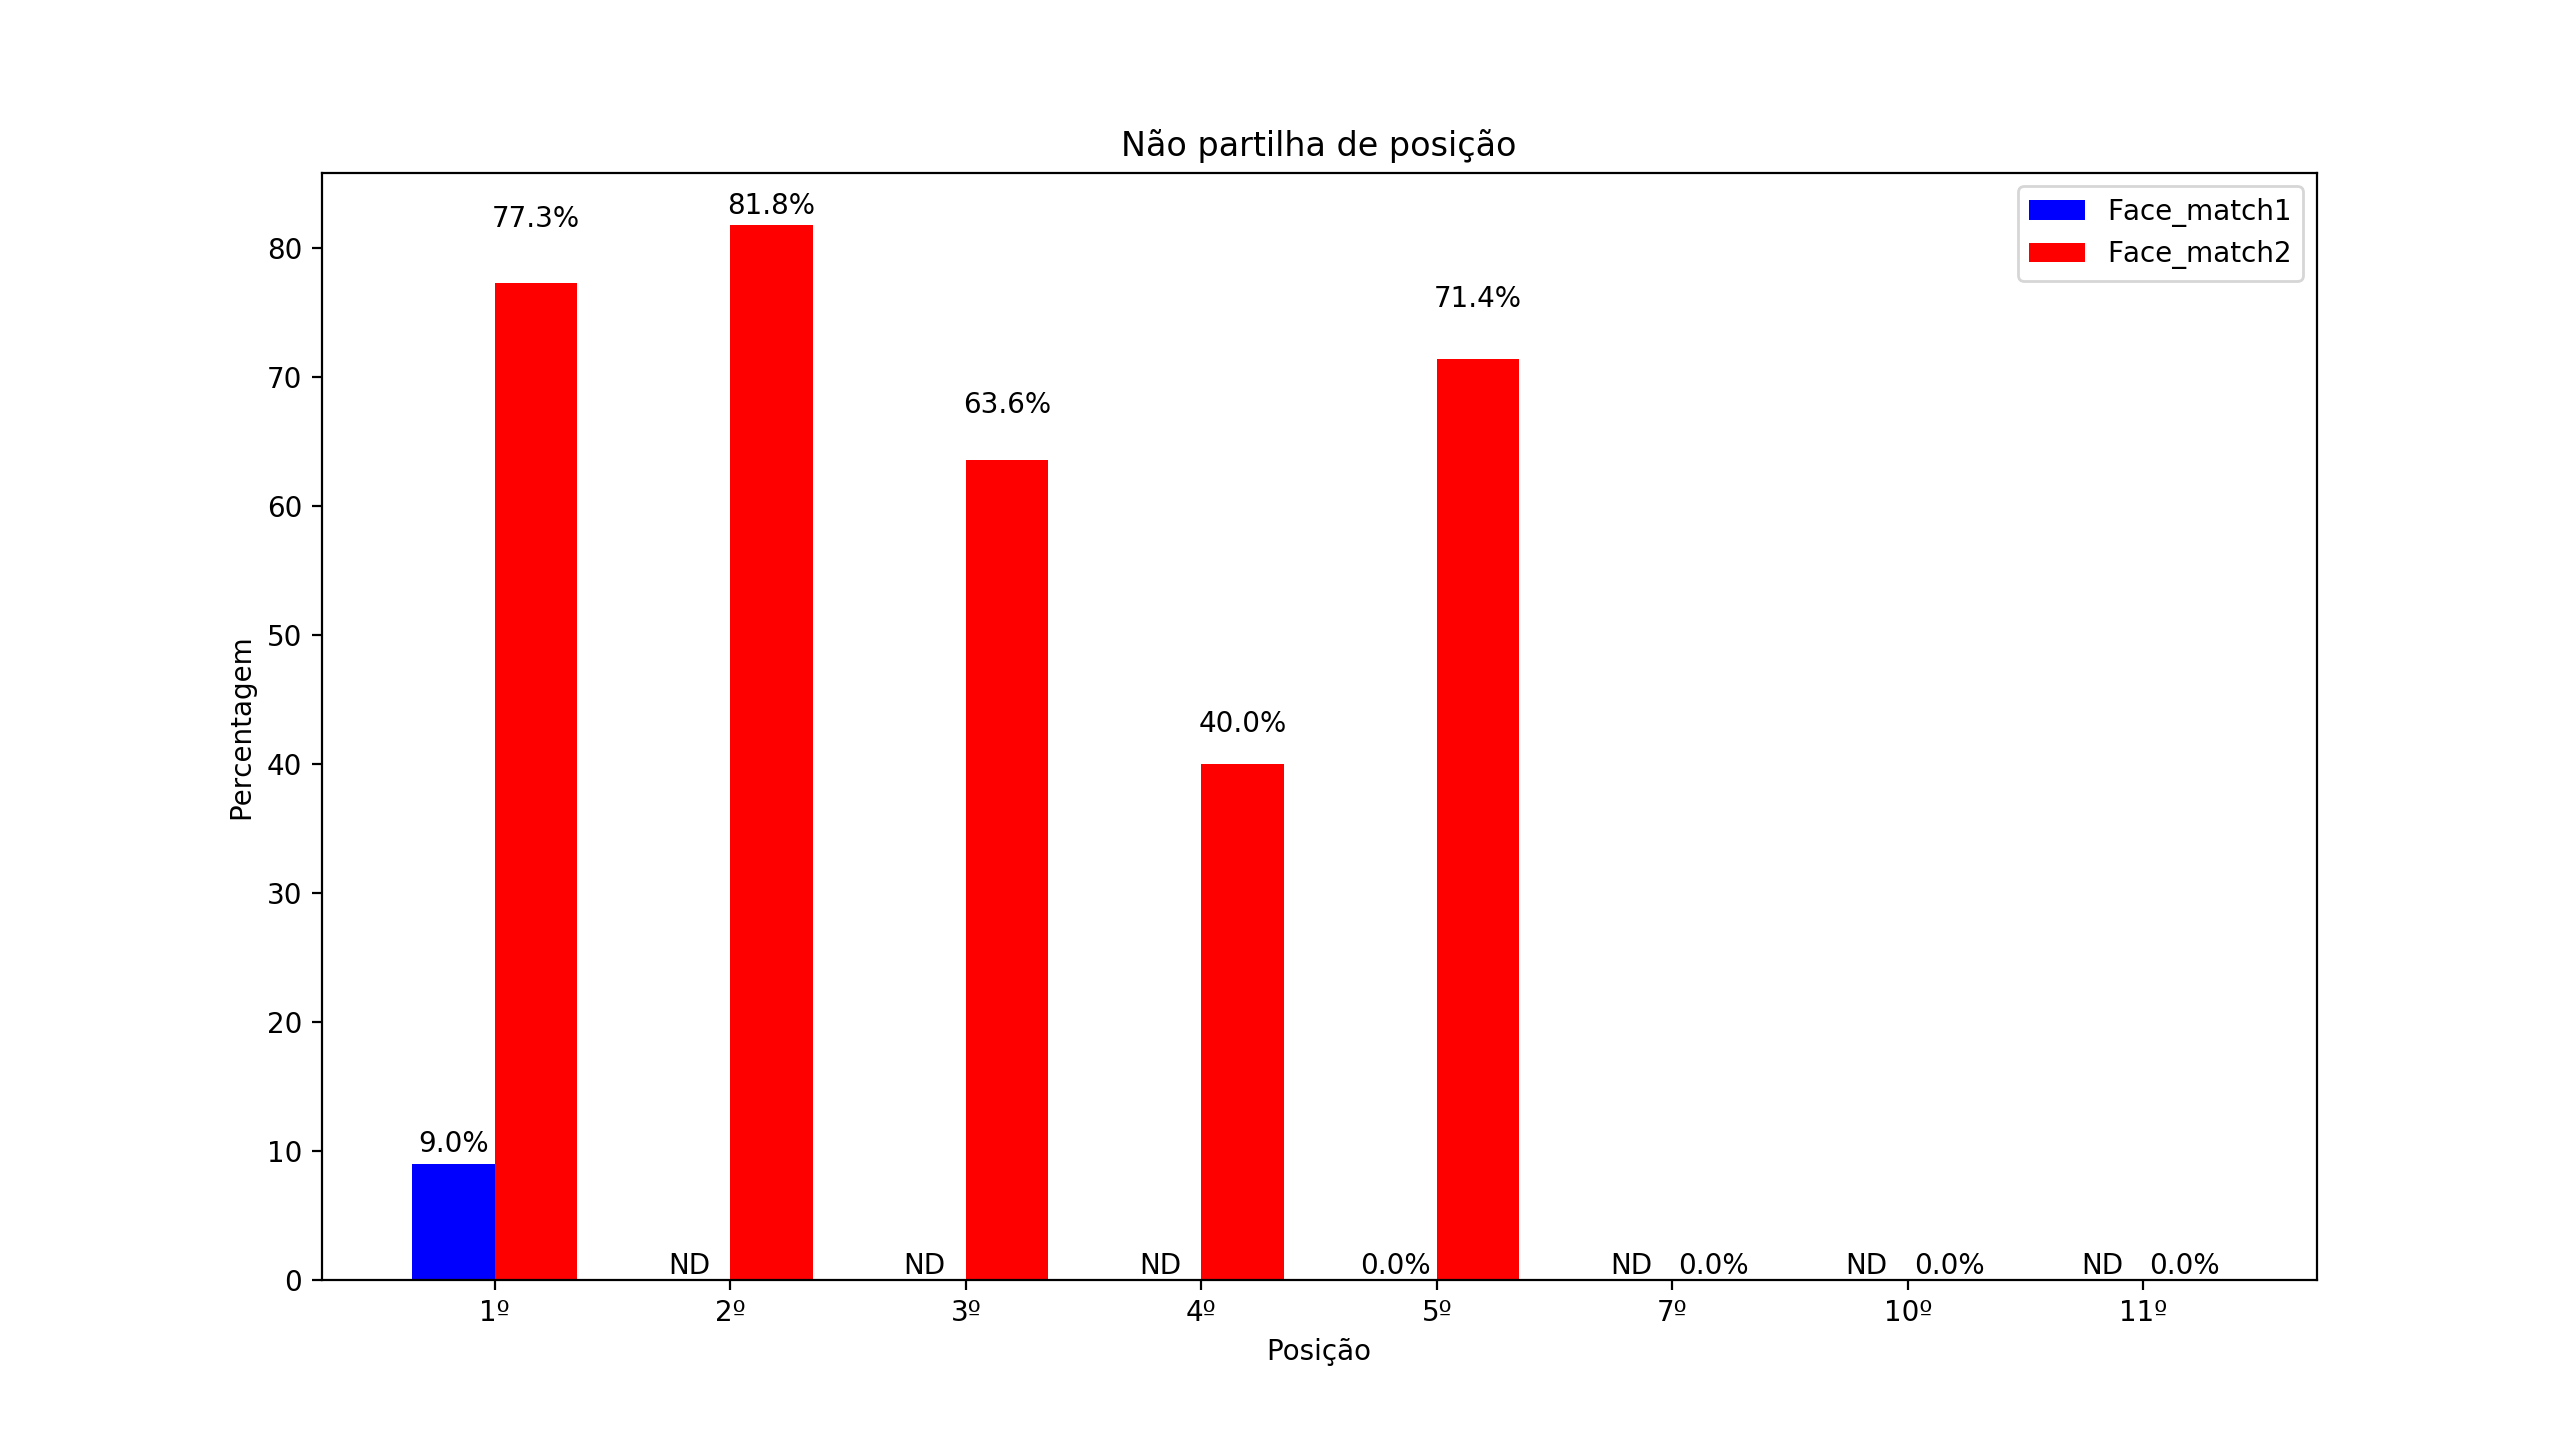
\includegraphics[width=15.0cm]{face_match_rankings2.png}
    \caption{}
  \end{subfigure}
  \caption{Acertos de cada solução (a) e a taxa de partilha de posições (b).}
  \label{fig:face_match_rankings}
\end{figure}

\newline
\noindent
\noindent Pela análise dos gráficos, é possível perceber que a solução que conjuga apenas duas imagens (Face\_match1) coloca o indivíduo certo na 1ª posição com maior frequência. Contudo, coloca também outros indivíduos, não sendo por isso a mais determinista.\newline
\noindent Por outro lado, a solução que opera sobre três imagens em simultâneo (Face\_match2), é menos certeira nas avaliações que faz, mas não apresenta o problema de colocar demasiadas pessoas numa mesma posição. \newline
\noindent De um modo geral, os casos em que a rede falhou prendem-se com os exemplos retratados na figura \ref{fig:falhas}. Quando o mesmo indivíduo possui imagens muitos distintas, é dada uma resposta negativa falsa. Por outro lado, quando são duas pessoas diferentes, mas parecidas, é dada uma resposta positiva falsa.

\begin{figure}[h]
  \centering
  \begin{subfigure}{4.5cm}
    \centering
\includegraphics[width=4.5cm]{ar_falha1.jpg}
    \caption{}
  \end{subfigure}
  \hspace{1em}
  \begin{subfigure}{6.8cm}
    \centering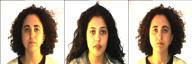
\includegraphics[width=6.8cm]{ar_falha2.jpg}
    \caption{}
  \end{subfigure}
  \caption{Casos típicos de falha.}
  \label{fig:falhas}
\end{figure}
\clearpage{\thispagestyle{empty}\cleardoublepage}
\chapter{Conclusões e Trabalho Futuro}
\label{chap:conc-trab-futuro}

\section{Conclusões Principais}
\label{sec:conc-princ}

Este trabalho serviu, acima de tudo, como uma introdução à temática das redes neuronais e respetiva implementação, para procurar dar resposta a alguns desafios. O conhecimento adquirido é e será mais valioso que qualquer resultado prático, formando uma base que se espera expandir no futuro.

\section{Trabalho Futuro}
\label{sec:trab-futuro}

De forma a suplementar o trabalho desenvolvido, algumas melhorias/adições podem ser destacadas:

\begin{enumerate}
    \item \textbf{Obter imagens com menos ruído (problema 1):} O facto de numa dada imagem de um indivíduo aparecerem, ora outros indivíduos ora partes dos corpos destes, não ajuda à avaliação das sequências. Muitas delas foram dadas como erradas, sendo que se tratavam da mesma pessoa (efeito indesejável do ruído existente).
    \item \textbf{Usar sequências com mais imagens (problema 2):} tendo observado as diferenças entre usar duas ou três imagens por sequência, o uso de mais imagens/combinações diferentes pode produzir resultados interessantes.
    \item \textbf{Alterar parâmetros/configurações na rede:} tal como descrito no capítulo \ref{chap3:sec:final}, certos parâmetros podem ter impacto no processo de aprendizagem de uma CNN e na performance sobre o conjunto de teste. Um modelo melhor contribui para um sistema de comparação de indivíduos melhor.
\end{enumerate}{}
\clearpage{\thispagestyle{empty}\cleardoublepage}

% SE EXISTIREM APENDICES, DESCOMENTAR O QUE ESTÁ EM BAIXO
% \appendix
% \include{apendice1}
% \clearpage{\pagestyle{empty}\cleardoublepage}
% \include{continuacao}
% \clearpage{\pagestyle{empty}\cleardoublepage}
% \include{apendice2}
% \clearpage{\pagestyle{empty}\cleardoublepage}
% \include{apendice3}
% \clearpage{\pagestyle{empty}\cleardoublepage}

\backmatter

\bibliographystyle{unsrt}
\bibliography{bibliografia}

\end{document}